\subsection{Memory layout in RAM}\label{sec:ram}\label{sec:mechanism}

With the index in memory, a query's time is set by where its nodes and points sit in the cache and translation hierarchy, not by how many it touches. This section prices every visit by depth (Figure~\ref{fig:depth}), then changes the layout under a fixed structure: page size, prefetching of child groups, and the leaf capacity on either page size.

\begin{figure*}[tb]
\centering
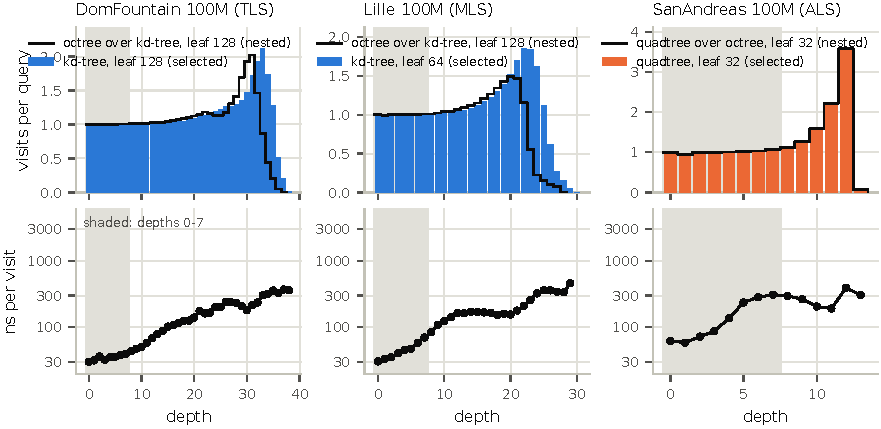
\includegraphics[width=\textwidth]{figures/fig_depth}
\caption{Visits per query (top) and nanoseconds per visit (bottom) by depth for the searched best structure of three 100M clouds, instrumented pass, sequential protocol. The shaded depths are the top eight levels. The nanoseconds of the instrumented pass include the telemetry and sum to about 1.25 times the timed latency; the shares between depths are what the figure is for.}
\label{fig:depth}
\end{figure*}

\paragraph{A visit costs 35\,ns at the top of a tree and 350 at a leaf.} On the DomFountain kd-tree a visit in the top eight levels costs \visitCostTopNs\,ns, one in the middle levels \visitCostMiddleNs\,ns and one in the deepest four \visitCostLeafNs\,ns: an order of magnitude within one tree. The top levels stay in cache for every query of a coherent trace and the deep levels do not. On the ground and mobile scans the top eight levels are \topLevelsShareDomFountain\% of a query's time; on the aerial terrain, where consecutive queries lie far apart, even the top levels miss and the leaves hold half the time.

\paragraph{Node counts do not predict time.} A least-squares model of latency on visited nodes, tested points and returned points, fitted per cloud on the instrumented search-half runs, predicts the gap from the octree default to the per-cloud best at a fraction of its size; adding box tests and tree size as terms does not repair it. One cloud makes the point: on DomFountain at 25M the octree default visits \exampleOctreeVisits{} nodes and tests \exampleOctreePoints{} points per query in \exampleOctreeUs\us, and the fastest structure, a \exampleOracleName, visits \exampleOracleVisits{} nodes and tests \exampleOraclePoints{} points in \exampleOracleUs\us, from a tree of \exampleOracleNodes{} million nodes against \exampleOctreeNodes{} million. More visits, more points, a third of the nodes, and a third less time. In memory no count the engine records ranks structures; only timing does.

\paragraph{Huge pages and prefetching.} Table~\ref{tab:layout} times a panel of structures (the searched best, the rule's picks, the library defaults and two wide structures) on three scenes at 25M and 100M under four variants of the same binary: as it is; with the node pool and point arrays on 2\,MB pages; with the next level prefetched when a child is pushed; and with both. Each ratio compares a structure with itself in the same process group. Huge pages speed up every tree, in proportion to its pool: \hugeSinglesHundredM$\times$ over the 100M structures, \hugeBigPools$\times$ for pools of 64\,MB or more against \hugeSmallPools$\times$ below, \hugeSinglesTwentyFiveM$\times$ at 25M, and down to \hugeMin$\times$ for the largest pool in the panel, a 10-million-node quadtree on SanAndreas (\hugeAloneQt$\times$ when that structure is timed alone). A 75\,MB pool is some 18\,000 pages of 4\,KiB against a second-level translation buffer of 1\,500 entries, so on small pages every cold visit pays a page walk on top of its cache miss, and the 2\,MB page removes it. Prefetching the next level helps the binary and four-way trees, whose pushed child group is one or two cache lines, by up to \prefetchMin$\times$, and hurts the 64-way hierarchical grid by \prefetchHGrid$\times$ on every cloud: its two-kilobyte child group is streamed by the box tests anyway and the prefetches are extra traffic. The two do not add (\bothSinglesHundredM$\times$ together), because they hide the same miss. These ratios were taken interleaved, with several large indexes resident; timed sequentially on the nine 100M clouds of Table~\ref{tab:panel}, huge pages give \panelHugeOverBaseSingles$\times$ (\panelHugeOverBaseSinglesMin{} to \panelHugeOverBaseSinglesMax), with the same ordering by pool size. The interleaved figure includes the translation-buffer pressure that co-resident indexes add; the sequential one is what a lone index gains.

\begin{table*}[t]
\centering\footnotesize
\caption{Layout variants over the unchanged binary, geometric mean (range) of per-structure latency ratios (below 1: the variant is faster), three scenes at 25M and 100M, interleaved in rotated process groups. Pools are the hot-node arrays at 32 bytes per node; the last row is the 64-way hierarchical grid and the variants built on it.}
\label{tab:layout}
% generated by scripts/paper/tables.py; do not edit
\begin{tabular}{lrrr}
\toprule
Structures (count) & huge pages\,/\,base & child prefetch\,/\,base & both\,/\,base \\
\midrule
100M points, all structures (17) & 0.915 (0.71--0.99) & 0.941 (0.72--1.12) & 0.928 (0.69--1.10) \\
100M points, node pool $\geq$ 64 MB (14) & 0.902 (0.71--0.97) & 0.911 (0.72--0.97) & 0.896 (0.69--0.97) \\
100M points, node pool $<$ 64 MB (3) & 0.978 (0.97--0.99) & 1.096 (1.08--1.12) & 1.094 (1.09--1.10) \\
25M points, all structures (17) & 0.974 (0.91--1.01) & 0.970 (0.90--1.10) & 0.970 (0.86--1.11) \\
hierarchical grid, 64-way (8) & 0.982 (0.97--1.01) & 1.092 (1.08--1.12) & 1.093 (1.08--1.11) \\
\bottomrule
\end{tabular}

\end{table*}

\paragraph{The interleaving penalty is translation reach.} The kd-tree timed alone is \aloneOverInterleavedKdBase$\times$ its interleaved time on small pages and \aloneOverInterleavedKdHuge$\times$ on huge pages, while the octree keeps a few percent either way (\aloneOverInterleavedOtBase{} and \aloneOverInterleavedOtHuge). For the memory-bound trees, timing several indexes in one process costs what their pages cost in the translation buffer, which is why every headline ratio of this paper is re-timed sequentially.

\paragraph{The leaf on both page sizes.} Table~\ref{tab:leaflever} sweeps the leaf capacity of the rule's two primitives from 16 to 1\,024 points on the nine 100M clouds, sequentially, on both page sizes. On 4\,KiB pages the kd-tree's best leaf is 64 or 128 on eight of the nine clouds; leaf 32 costs \leafKdOverThirtyTwoBase$\times$ the best and leaf 128 \leafKdOverHundredTwentyEightBase$\times$. On huge pages the best leaf moves down in \leafShiftPairs{} of \leafPairs{} cloud--primitive pairs, all but one of them kd-trees, to 16 or 32 points on five clouds; the small-leaf penalty halves to \leafKdOverThirtyTwoHuge$\times$ and leaf 128 now costs \leafKdOverHundredTwentyEightHuge$\times$. The quadtree wants a larger leaf, 128 to 512 points on the aerial scenes, and its leaf-128 pick stays within \leafQtOverHundredTwentyEightBase$\times$ of the best in either mode, while leaf 32 costs it \leafQtOverThirtyTwoBase$\times$. The worst leaf of the sweep costs \leafWorstMin{} to \leafWorstMax$\times$ the best. The leaf is a lever of the same order as the primitive, its optimum depends on the page size as much as on the structure, and the rule's 64 to 128 is a safe choice on either.

\begin{table*}[t]
\centering\footnotesize
\caption{The leaf capacity on nine 100M clouds, sequential protocol, 4\,KiB and 2\,MB pages: the best leaf per cloud (count of clouds), and the latency at leaf 32, at leaf 128 and at the worst leaf of the sweep over the latency at the best leaf, geometric mean (range).}
\label{tab:leaflever}
% generated by scripts/paper/tables.py; do not edit
\begin{tabular}{llllrr}
\toprule
Primitive & Pages & best leaf (cells) & leaf 32\,/\,best & leaf 128\,/\,best & worst\,/\,best \\
\midrule
kd-tree, sliding midpoint & 4 KiB & 16 (1), 64 (4), 128 (4) & 1.076 (1.02--1.18) & 1.013 (1.00--1.04) & 1.557 (1.40--1.77) \\
 & 2 MB & 16 (3), 32 (2), 64 (1), 128 (3) & 1.040 (1.00--1.14) & 1.036 (1.00--1.10) & 1.576 (1.40--1.83) \\
quadtree, points' centre & 4 KiB & 64 (2), 128 (2), 256 (3), 512 (2) & 1.315 (1.03--1.86) & 1.037 (1.00--1.14) & 1.689 (1.41--2.50) \\
 & 2 MB & 64 (1), 128 (3), 256 (3), 512 (2) & 1.297 (1.03--1.81) & 1.037 (1.00--1.11) & 1.691 (1.41--2.47) \\
\bottomrule
\end{tabular}

\end{table*}

% PENDING (battery 2x, results/eval_traces/threads_makinon2): page-blocked against depth-first node order in RAM,
% single-threaded and at 18/36 threads, both page sizes.
